\chapter{Oksidasi dan Reduksi dalam Kimia Organik}\label{ch:b1:organic-redox}

Sebotol anggur yang dibiarkan terbuka berubah, dalam beberapa hari,
menjadi cuka: bakteri memakai oksigen udara untuk mengoksidasi etanol
menjadi asam etanoat. Sebuah keton dan alkohol asalnya berbeda dua atom
hidrogen --- dan, jika dihitung dengan benar, dua elektron. Oksidasi dan
reduksi organik tidak tampak seperti pertukaran elektron antara ion-ion
logam dalam \cref{ch:b1:nernst}, karena elektron berpindah bersama proton
atau bersama ion hidrida, tetapi pembukuannya sama. Bab ini memberikan
\omterm{def:b1:organic-redox:oxidation-level}{tingkat oksidasi} kepada karbon, memakainya untuk meramalkan apa yang
dihasilkan setiap alkohol jika dioksidasi, dan memperkenalkan pereaksi
hidrida yang mereduksi senyawa karbonil, dengan memperhatikan gugus mana
yang dibiarkan utuh oleh setiap pereaksi.

\begin{recall}
\omterm{def:b1:nernst:oxidation-number}{Bilangan oksidasi}, \omterm{def:b1:nernst:couple}{setengah reaksi}, dan penyetaraan persamaan redoks
terdapat dalam \cref{ch:b1:nernst}; kelas alkohol dan kelas karbon dalam
\cref{ch:b1:electronic-effects}; \omterm{def:b1:acetals-protection:hemiacetal}{asetal} dan \omterm{def:b1:acetals-protection:protecting-group}{proteksi} gugus karbonil dalam
\cref{ch:b1:acetals-protection}; adisi Grignard dalam
\cref{ch:b1:organomagnesium}.
\end{recall}

\begin{omfigure}
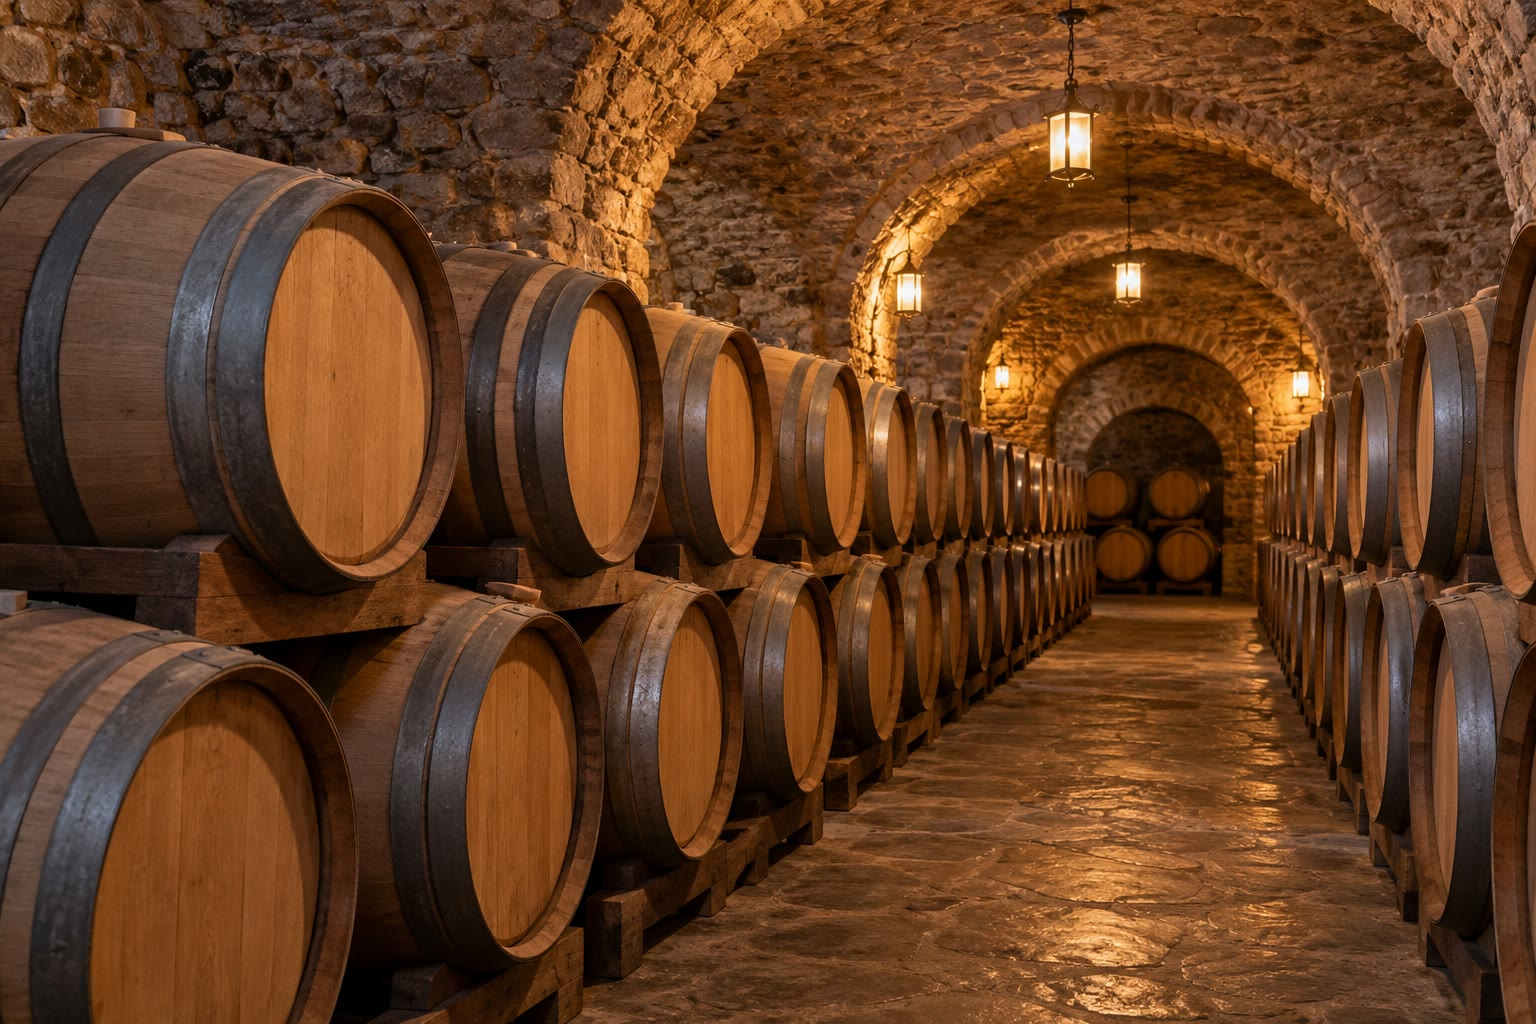
\includegraphics[width=0.58\linewidth]{images/book2/ai/b1-24-wine-cellar.jpg}

{\small Anggur yang dimatangkan di dalam ruang bawah tanah. Jika terhindar
dari udara, anggur mempertahankan etanolnya; jika terpapar udara, bakteri
asam asetat mengoksidasinya menjadi asam etanoat.}
\end{omfigure}

\section{Tingkat oksidasi karbon}

\begin{definition}[Tingkat oksidasi]\label{def:b1:organic-redox:oxidation-level}
\emph{Tingkat oksidasi}\index{tingkat oksidasi} sebuah atom karbon adalah
\omterm{def:b1:nernst:oxidation-number}{bilangan oksidasinya}, yang diperoleh dengan aturan dalam
\cref{prop:b1:nernst:on-rules}: setiap ikatan dengan atom yang lebih
elektronegatif (O, N, halogen) dihitung $+1$, setiap ikatan dengan
hidrogen $-1$, setiap ikatan dengan karbon lain 0 (ikatan rangkap dua
dihitung dua kali).
\end{definition}

\begin{proposition}[Bilangan oksidasi karbon]\label{prop:b1:organic-redox:on-of-carbon}
\omterm{def:b1:nernst:oxidation-number}{Bilangan oksidasi} sebuah karbon sama dengan (banyaknya ikatan dengan O, N,
atau halogen) dikurangi (banyaknya ikatan dengan H). Dalam satu keluarga
senyawa dengan kerangka karbon yang sama, alkohol $\to$ aldehida atau
keton $\to$ asam karboksilat $\to$ karbon dioksida adalah deret oksidasi
yang masing-masing melibatkan dua elektron.
\end{proposition}

\begin{proof}
Putuskan setiap ikatan dan berikan kedua elektronnya kepada pasangan yang
lebih elektronegatif: dari H (kurang elektronegatif daripada C) karbon
memperoleh sebuah elektron, muatan $-1$ per C--H; kepada O, N, halogen
(lebih elektronegatif) karbon kehilangan satu, $+1$ per ikatan; ikatan
C--C dibagi sama rata. Dari \ce{-CH2OH} ($-1$ untuk karbon yang terikat
pada satu karbon lain) ke \ce{-CHO} ($+1$) ke \ce{-COOH} ($+3$), bilangan
itu naik 2 pada setiap tahap: dua elektron.
\end{proof}

\begin{omfigure}
\begin{tikzpicture}[font=\small, >={Stealth}]
  \foreach \x/\f/\n in {0/\ce{CH4}/-4, 2.4/\ce{CH3OH}/-2, 4.8/\ce{HCHO}/0, 7.2/\ce{HCOOH}/+2, 9.6/\ce{CO2}/+4} {
    \node[draw, rounded corners, minimum width=1.5cm] at (\x,0) {\f};
    \node[below] at (\x,-0.5) {$\n$};
  }
  \foreach \x in {0.8,3.2,5.6,8.0} \draw[->, thick, omThm] (\x,0) -- ++(0.8,0);
  \node[omThm, above] at (4.8,0.5) {oksidasi: $-2\,\mathrm{e^-}$ (dan $-2\,\ce{H+}$) pada setiap tahap};
  \node[left] at (-0.9,-0.75) {biloks C:};
\end{tikzpicture}

{\small \omterm{def:b1:organic-redox:oxidation-level}{Tingkat oksidasi} keluarga satu karbon: metana, metanol, metanal,
asam metanoat, karbon dioksida. Setiap panah adalah oksidasi dua elektron;
jika dibaca mundur, sebuah reduksi.}
\end{omfigure}

\begin{method}[Menyetarakan setengah reaksi organik]\label{met:b1:organic-redox:balance-organic-redox}
\begin{enumerate}
  \item Tuliskan \omterm{def:b1:nernst:couple}{oksidator} dan \omterm{def:b1:nernst:couple}{reduktor} organiknya dengan kerangka yang
        sama.
  \item Hitunglah elektronnya dari perubahan \omterm{def:b1:nernst:oxidation-number}{bilangan oksidasi} karbon yang
        berubah (atau secara sederhana: dua untuk setiap pasang H yang
        hilang, atau untuk setiap O yang bertambah).
  \item Setarakan oksigen dengan air, hidrogen dengan \ce{H+}, dan muatan
        dengan elektron.
\end{enumerate}
Etanol menjadi asam etanoat: \ce{CH3CH2OH + H2O -> CH3COOH + 4H+ + 4e-}.
Dengan dikromat yang diasamkan (\ce{Cr2O7^2- + 14H+ + 6e- -> 2Cr^3+ + 7H2O}),
tiga molekul etanol untuk dua ion dikromat:
\ce{3CH3CH2OH + 2Cr2O7^2- + 16H+ -> 3CH3COOH + 4Cr^3+ + 11H2O}.
\end{method}

\section{Mengoksidasi alkohol}

\begin{proposition}[Hasil oksidasi alkohol]\label{prop:b1:organic-redox:alcohol-oxidation}
Alkohol primer \ce{RCH2OH} dioksidasi menjadi aldehida \ce{RCHO}, lalu
(dalam air, dengan \omterm{def:b1:nernst:couple}{oksidator} kuat) menjadi asam karboksilat \ce{RCOOH};
alkohol sekunder \ce{R2CHOH} menjadi keton \ce{R2CO}, yang tahan terhadap
oksidasi lebih lanjut; alkohol tersier \ce{R3COH} tidak teroksidasi tanpa
memutus sebuah ikatan C--C.
\end{proposition}

\begin{proof}
Oksidasi alkohol melepaskan hidrogen OH dan sebuah hidrogen dari karbon
karbinol, sehingga terbentuk C=O. Karbon karbinol tersier tidak mempunyai
hidrogen semacam itu. Aldehida masih membawa sebuah H pada karbon
karbonilnya; dalam air aldehida itu sebagian terhidrasi, \ce{RCH(OH)2},
yang dioksidasi lagi dengan cara yang sama menjadi \ce{RCOOH}. Keton tidak
mempunyai H pada karbon itu dan berhenti.
\end{proof}

\omterm{def:b1:nernst:couple}{Oksidator} kuat dalam air --- kalium dikromat atau permanganat yang
diasamkan --- mengoksidasi alkohol primer menjadi asam. Untuk berhenti
pada aldehida, aldehida itu didistilasi keluar segera setelah terbentuk
(aldehida mendidih pada suhu yang lebih rendah daripada alkohol asalnya,
karena tidak mempunyai \omterm{def:b1:intermolecular-forces-solvents:hbond}{ikatan hidrogen} O--H), atau dipakai pereaksi
anhidrat yang lebih lunak, yang diuraikan dalam jilid Tahun~2.

\begin{safety}{\ghs[5mm]{GHS03}\,\ghs[5mm]{GHS05}\,\ghs[5mm]{GHS06}\,\ghs[5mm]{GHS07}\,\ghs[5mm]{GHS08}\,\ghs[5mm]{GHS09}}
Kalium dikromat, \omterm{def:b1:nernst:couple}{oksidator} jingga yang klasik untuk alkohol, digolongkan
di antara zat yang dapat menyebabkan kanker: zat itu hanya ditangani
dalam jumlah kecil, dengan sarung tangan dan kacamata pelindung, dan
limbah kromiumnya dikumpulkan secara terpisah; bila mungkin, \omterm{def:b1:nernst:couple}{oksidator}
yang kurang berbahaya lebih disukai.
% ledger: ghs:K2Cr2O7
\end{safety}

\section{Mereduksi senyawa karbonil dengan hidrida}

\begin{definition}[Donor hidrida]\label{def:b1:organic-redox:hydride-donor}
\emph{Donor hidrida}\index{donor hidrida} memindahkan sebuah atom hidrogen
beserta \omterm{def:b1:lewis-resonance-vsepr:lewis}{pasangan ikatannya}, \ce{H-}, ke karbon yang elektrofilik. Natrium
borohidrida \ce{NaBH4} dan litium aluminium hidrida \ce{LiAlH4} adalah
\emph{hidrida logam kompleks}\index{hidrida logam kompleks}: hidridanya
diserahkan dari ion \ce{BH4-} atau \ce{AlH4-}, bukan sebagai ion bebas.
\end{definition}

\begin{omfigure}
\setchemfig{atom sep=2.1em}
\schemestart
\chemfig{H_3B^{-}-[@{bh}]@{h}H}
\+
\chemfig{@{c}C(-[:150]R)(-[:210]R')=[@{co}]@{o}O}
\arrow{->}
\chemfig{C(-[:150]R)(-[:210]R')(-[2]H)-O^{-}}
\arrow{->[\ce{H2O}]}
\chemfig{C(-[:150]R)(-[:210]R')(-[2]H)-OH}
\schemestop
\chemmove{\draw[->, thick, shorten <=2pt, shorten >=3pt](bh) .. controls +(80:9mm) and +(180:7mm) .. (c);
          \draw[->, thick, shorten <=2pt, shorten >=2pt](co) .. controls +(90:6mm) and +(90:6mm) .. (o);}
\par\vspace{6pt}

{\small Reduksi keton oleh borohidrida: sepasang elektron B--H membentuk
ikatan C--H yang baru sementara pasangan $\pi$ C=O berpindah ke oksigen;
\omterm{def:b1:alcohol-activation:alkoxide}{alkoksidanya} diprotonasi oleh pelarut (air atau alkohol) atau pada
pengolahan akhir. Setiap \ce{BH4-} dapat menyerahkan keempat hidrogennya
secara bergiliran.}
\end{omfigure}

\begin{proposition}[Cakupan kedua hidrida]\label{prop:b1:organic-redox:hydride-scope}
Natrium borohidrida, yang dipakai dalam air atau alkohol, mereduksi
aldehida menjadi alkohol primer dan keton menjadi alkohol sekunder, dan
membiarkan ester, asam karboksilat, amida, dan ikatan rangkap dua C=C
tetap utuh. Litium aluminium hidrida, yang dipakai dalam eter kering,
juga mereduksi ester dan asam karboksilat menjadi alkohol primer, dan
bereaksi hebat dengan air.
\end{proposition}

\begin{proof}
Ikatan Al--H lebih terpolarisasi daripada ikatan B--H (aluminium kurang
elektronegatif daripada boron), sehingga \ce{AlH4-} adalah \omterm{def:b1:organic-redox:hydride-donor}{donor hidrida}
yang jauh lebih kuat, yang mampu menyerang karbonil ester dan karboksilat
yang kurang elektrofilik; reaktivitas yang sama membuatnya bereaksi
dengan hidrogen asam apa pun, termasuk air. \ce{BH4-} hanya bereaksi
lambat dengan air dan alkohol, dan hanya menyerang karbonil yang paling
elektrofilik. Ikatan C=C yang terisolasi tidak elektrofilik dan tidak
direduksi oleh keduanya.
\end{proof}

\section{Selektivitas}

\begin{definition}[Reaksi kemoselektif]\label{def:b1:organic-redox:chemoselective}
\emph{Reaksi kemoselektif}\index{reaksi kemoselektif} bekerja pada satu
gugus fungsi sebuah molekul dengan adanya gugus lain yang, dengan pereaksi
yang berbeda, dapat ikut bereaksi.
\end{definition}

\begin{omfigure}
\begin{tabular}{lcc}
\hline
gugus & \ce{NaBH4} (pelarut alkohol) & \ce{LiAlH4} (eter kering) \\
\hline
aldehida \ce{RCHO} & alkohol primer & alkohol primer \\
keton \ce{R2CO} & alkohol sekunder & alkohol sekunder \\
ester \ce{RCOOR} & tidak bereaksi & dua alkohol \\
asam karboksilat \ce{RCOOH} & tidak bereaksi (garam) & alkohol primer \\
alkena \ce{C=C} & tidak bereaksi & tidak bereaksi \\
\omterm{def:b1:acetals-protection:hemiacetal}{asetal} & tidak bereaksi & tidak bereaksi \\
\hline
\end{tabular}

\smallskip
{\small Apa yang direduksi oleh kedua hidrida. Natrium borohidrida adalah
pereaksi yang kemoselektif; litium aluminium hidrida, pereaksi yang kuat.}
\end{omfigure}

\begin{example}[Sebuah keto ester]\label{ex:b1:organic-redox:ketoester}
Etil 4-oksopentanoat, \ce{CH3CO(CH2)2COOEt}, dengan natrium borohidrida
menghasilkan etil 4-hidroksipentanoat: hanya ketonnya yang direduksi.
Dengan litium aluminium hidrida, kedua gugus direduksi: pentana-1,4-diol
(dan etanol). Untuk mereduksi esternya saja, ketonnya harus lebih dahulu
diproteksi sebagai \omterm{def:b1:acetals-protection:hemiacetal}{asetal} (\cref{ch:b1:acetals-protection}).
\end{example}

\begin{inthelab}[Mereduksi sebuah keton]
Natrium borohidrida ditambahkan sedikit demi sedikit ke dalam larutan
keton yang dingin dalam etanol: reaksinya eksoterm, dan hidrogen
menggelembung dari reaksi lambat pereaksi itu dengan pelarutnya. Sesudah
diaduk, asam encer merusak pereaksi yang berlebih (hidrogen lagi: tidak
boleh ada nyala api di dekatnya) dan alkoholnya diekstraksi. Sebaliknya,
litium aluminium hidrida hanya dipakai dalam eter kering di bawah gas
inert, dan kelebihannya dirusak dengan sangat hati-hati.
\end{inthelab}

\section{Latihan}

\begin{exercise}[$\star$]\label{exo:b1:organic-redox:1}
Tentukan \omterm{def:b1:nernst:oxidation-number}{bilangan oksidasi} setiap karbon dalam etanol, etanal, asam
etanoat, propanon, dan asam metanoat.
\end{exercise}

\begin{exercise}[$\star$]\label{exo:b1:organic-redox:2}
Apa yang dihasilkan dikromat yang diasamkan dengan propan-1-ol,
propan-2-ol, dan 2-metilpropan-2-ol?
\end{exercise}

\begin{exercise}[$\star$]\label{exo:b1:organic-redox:3}
Tuliskan \omterm{def:b1:nernst:couple}{setengah reaksi} pasangan propanon/propan-2-ol dan etanal/etanol
dalam asam.
\end{exercise}

\begin{exercise}[$\star$]\label{exo:b1:organic-redox:4}
Apa yang dihasilkan natrium borohidrida dan litium aluminium hidrida
dengan butanal, butanon, etil butanoat, dan asam butanoat?
\end{exercise}

\begin{exercise}[$\star\star$]\label{exo:b1:organic-redox:5}
Setarakan oksidasi propan-2-ol oleh permanganat dalam asam
(\ce{MnO4-}/\ce{Mn^2+}) dan hitunglah volume permanganat
\qty{0.020}{mol/L} yang diperlukan untuk \qty{1.20}{g} alkohol ($M = \qty{60.0}{g/mol}$).
\end{exercise}

\begin{exercise}[$\star\star$]\label{exo:b1:organic-redox:6}
Bagaimana propanal dapat diperoleh dari propan-1-ol tanpa teroksidasi
lebih lanjut? Gunakan titik didihnya: propan-1-ol \qty{97}{\celsius},
propanal \qty{48}{\celsius}.
% ledger: bp:propanal, bp:propan-1-ol
\end{exercise}

\begin{exercise}[$\star\star$]\label{exo:b1:organic-redox:7}
Tuliskan mekanisme reduksi etanal oleh \ce{BH4-} dalam etanol. Atom
manakah dalam produknya yang berasal dari pereaksi?
\end{exercise}

\begin{exercise}[$\star\star$]\label{exo:b1:organic-redox:8}
Reduksi butan-2-on dengan \ce{NaBH4} menghasilkan alkohol yang \omterm{def:b1:stereochemistry-in-depth:stereocentre}{kiral}.
Apakah alkohol itu aktif optis? Mengapa?
\end{exercise}

\begin{exercise}[$\star\star$]\label{exo:b1:organic-redox:9}
Dalam uji napas alkohol yang dahulu dipakai polisi, dikromat yang jingga
berubah menjadi hijau. Tuliskan reaksinya dengan etanol dan jelaskan
perubahan warnanya.
\end{exercise}

\begin{exercise}[$\star\star\star$]\label{exo:b1:organic-redox:10}
Usulkan sintesis: 2-metilbutan-2-ol dari etanal dan sebuah \omterm{def:b1:organomagnesium:organometallic}{pereaksi
Grignard}, diikuti oksidasi dan tahap Grignard kedua; pentan-3-ol dari
propanal. Hitunglah banyaknya oksidasi dan reduksi.
\end{exercise}

\begin{exercise}[$\star\star\star$]\label{exo:b1:organic-redox:11}
Dalam metil 4-oksopentanoat, \ce{CH3CO(CH2)2COOCH3}, reduksilah hanya gugus
esternya. Rencanakan ketiga tahapnya dengan sebuah \omterm{def:b1:acetals-protection:protecting-group}{proteksi}
dan tentukan produknya.
\end{exercise}

\begin{exercise}[$\star\star\star$]\label{exo:b1:organic-redox:12}
Tunjukkan bahwa pada oksidasi alkohol primer menjadi asam, empat elektron
dipertukarkan, melalui \omterm{def:b1:nernst:oxidation-number}{bilangan oksidasi} dan melalui \omterm{def:b1:nernst:couple}{setengah reaksinya}.
Perumumlah untuk oksidasi metana menjadi karbon dioksida.
\end{exercise}

\section{Soal: Dari Sikloheksanol ke Asam Adipat}

\begin{problem}[{Soal akhir pekan --- tingkat oksidasi dalam sikloheksanol,
sikloheksanon, dan asam adipat, oksidasi oleh asam nitrat beserta
elektronnya, sebuah jalan dengan hidrogen peroksida, dan massa dinitrogen
oksida yang dilepaskan per ton asam adipat}]
\label{pb:b1:organic-redox:1}
Asam adipat, asam heksanadioat \ce{HOOC(CH2)4COOH}, dibuat dalam skala
besar untuk nilon, sebagian besar melalui oksidasi sikloheksanol (bersama
sikloheksanon) oleh asam nitrat, yang melepaskan dinitrogen oksida
\ce{N2O}, sebuah gas rumah kaca yang kuat. Massa molar (\unit{g/mol}):
\ce{C6H12O} 100.0, \ce{C6H10O} 98.0, \ce{C6H10O4} 146.0, \ce{N2O} 44.0,
\ce{HNO3} 63.0, \ce{H2O2} 34.0.

\medskip
\noindent\textbf{Bagian I --- \omterm{def:b1:organic-redox:oxidation-level}{Tingkat oksidasi}.}
\begin{enumerate}
  \item Tentukan \omterm{def:b1:nernst:oxidation-number}{bilangan oksidasi} setiap karbon sikloheksanol.
  \item Sama halnya untuk sikloheksanon.
  \item Sama halnya untuk asam adipat.
  \item Karbon manakah yang teroksidasi dari sikloheksanol menjadi asam
        adipat, dan ikatan manakah yang putus?
  \item Berapa elektron yang dilepaskan oleh satu molekul sikloheksanol?
  \item Mengapa sikloheksanon, sebuah keton, tetap teroksidasi lebih lanjut
        di sini?
\end{enumerate}

\medskip
\noindent\textbf{Bagian II --- Jalan asam nitrat.}
\begin{enumerate}[resume]
  \item Tuliskan \omterm{def:b1:nernst:couple}{setengah reaksi} sikloheksanol menjadi asam adipat dalam
        asam.
  \item Tentukan \omterm{def:b1:nernst:oxidation-number}{bilangan oksidasi} N dalam \ce{HNO3} dan dalam \ce{N2O}.
  \item Tuliskan \omterm{def:b1:nernst:couple}{setengah reaksi} \ce{HNO3}/\ce{N2O}.
  \item Gabungkan keduanya; periksalah bahwa diperoleh
        \ce{C6H12O + 2HNO3 -> C6H10O4 + N2O + 2H2O}.
  \item Berapa mol elektron yang dipertukarkan per mol asam adipat?
  \item Hitunglah massa asam nitrat yang terpakai per ton asam adipat.
\end{enumerate}

\medskip
\noindent\textbf{Bagian III --- Jalan dengan hidrogen peroksida.}
\begin{enumerate}[resume]
  \item Tuliskan \omterm{def:b1:nernst:couple}{setengah reaksi} \ce{H2O2}/\ce{H2O}.
  \item Tuliskan dan setarakan oksidasi sikloheksanol oleh hidrogen
        peroksida menjadi asam adipat.
  \item Hitunglah massa \ce{H2O2} per ton asam adipat.
  \item Apa satu-satunya produk sampingnya? Mengapa jalan ini disebut
        lebih hijau?
  \item Hidrogen peroksida harus diaktifkan oleh \omterm{def:b1:elementary-steps:catalyst}{katalis}. Dengan memakai
        \cref{exo:b1:nernst:12}, jelaskan mengapa oksidasi yang disukai
        secara termodinamika masih dapat memerlukan \omterm{def:b1:elementary-steps:catalyst}{katalis}.
  \item Apa yang akan dilakukan natrium borohidrida terhadap
        sikloheksanon? Tuliskan reaksinya.
\end{enumerate}

\medskip
\noindent\textbf{Bagian IV --- Massa dan gas rumah kaca.}
\begin{enumerate}[resume]
  \item Hitunglah jumlah asam adipat dalam satu ton.
  \item Hitunglah jumlah \ce{N2O} yang terbentuk bersamanya melalui jalan
        nitrat.
  \item Hitunglah massa sikloheksanol yang diperlukan per ton, pada
        \omterm{def:b1:extent-q-and-k:fractional-extent}{rendemen} \qty{95}{\percent}.
  \item Nyatakan massa \ce{N2O} yang dilepaskan per ton asam adipat
        melalui jalan nitrat, dalam ton.
\end{enumerate}
\end{problem}
